\documentclass[]{book}
\usepackage{lmodern}
\usepackage{amssymb,amsmath}
\usepackage{ifxetex,ifluatex}
\usepackage{fixltx2e} % provides \textsubscript
\ifnum 0\ifxetex 1\fi\ifluatex 1\fi=0 % if pdftex
  \usepackage[T1]{fontenc}
  \usepackage[utf8]{inputenc}
\else % if luatex or xelatex
  \ifxetex
    \usepackage{mathspec}
  \else
    \usepackage{fontspec}
  \fi
  \defaultfontfeatures{Ligatures=TeX,Scale=MatchLowercase}
\fi
% use upquote if available, for straight quotes in verbatim environments
\IfFileExists{upquote.sty}{\usepackage{upquote}}{}
% use microtype if available
\IfFileExists{microtype.sty}{%
\usepackage{microtype}
\UseMicrotypeSet[protrusion]{basicmath} % disable protrusion for tt fonts
}{}
\usepackage{hyperref}
\hypersetup{unicode=true,
            pdftitle={PDOK LocatieServer},
            pdfauthor={Willy Tadema},
            pdfborder={0 0 0},
            breaklinks=true}
\urlstyle{same}  % don't use monospace font for urls
\usepackage{natbib}
\bibliographystyle{apalike}
\usepackage{longtable,booktabs}
\usepackage{graphicx,grffile}
\makeatletter
\def\maxwidth{\ifdim\Gin@nat@width>\linewidth\linewidth\else\Gin@nat@width\fi}
\def\maxheight{\ifdim\Gin@nat@height>\textheight\textheight\else\Gin@nat@height\fi}
\makeatother
% Scale images if necessary, so that they will not overflow the page
% margins by default, and it is still possible to overwrite the defaults
% using explicit options in \includegraphics[width, height, ...]{}
\setkeys{Gin}{width=\maxwidth,height=\maxheight,keepaspectratio}
\IfFileExists{parskip.sty}{%
\usepackage{parskip}
}{% else
\setlength{\parindent}{0pt}
\setlength{\parskip}{6pt plus 2pt minus 1pt}
}
\setlength{\emergencystretch}{3em}  % prevent overfull lines
\providecommand{\tightlist}{%
  \setlength{\itemsep}{0pt}\setlength{\parskip}{0pt}}
\setcounter{secnumdepth}{5}
% Redefines (sub)paragraphs to behave more like sections
\ifx\paragraph\undefined\else
\let\oldparagraph\paragraph
\renewcommand{\paragraph}[1]{\oldparagraph{#1}\mbox{}}
\fi
\ifx\subparagraph\undefined\else
\let\oldsubparagraph\subparagraph
\renewcommand{\subparagraph}[1]{\oldsubparagraph{#1}\mbox{}}
\fi

%%% Use protect on footnotes to avoid problems with footnotes in titles
\let\rmarkdownfootnote\footnote%
\def\footnote{\protect\rmarkdownfootnote}

%%% Change title format to be more compact
\usepackage{titling}

% Create subtitle command for use in maketitle
\providecommand{\subtitle}[1]{
  \posttitle{
    \begin{center}\large#1\end{center}
    }
}

\setlength{\droptitle}{-2em}

  \title{PDOK LocatieServer}
    \pretitle{\vspace{\droptitle}\centering\huge}
  \posttitle{\par}
    \author{Willy Tadema}
    \preauthor{\centering\large\emph}
  \postauthor{\par}
    \date{}
    \predate{}\postdate{}
  
\usepackage{booktabs}

\begin{document}
\maketitle

{
\setcounter{tocdepth}{1}
\tableofcontents
}
\hypertarget{inleiding}{%
\chapter*{Inleiding}\label{inleiding}}
\addcontentsline{toc}{chapter}{Inleiding}

Dit is een handleiding voor \textbf{PDOK LocatieServer}.

De inhoud van deze handleiding is eerder gepubliceerd als onderdeel van de web API workshops van Willy Tadema, Niene Boeijen en The Green Land bij de provincie Zuid-Holland\footnote{\url{https://github.com/FrieseWoudloper/web-api-workshop}} en Gelderland\footnote{\url{https://github.com/FrieseWoudloper/web-api-workshop-gelderland}}.

In deze handleiding staan veel webservice requests. Deze requests kun je zelf uitproberen. Dat kun je in een internet browser doen, bijvoorbeeld in Google Chrome. Maar het kan ook handig zijn om een tool als Postman te gebruiken. Hoe je Postman installeert en de collectie met alle voorbeelden importeert, lees je in paragraaf \ref{postman}.

\hypertarget{intro}{%
\chapter{PDOK LocatieServer}\label{intro}}

PDOK staat voor \textbf{Publieke Dienstverlening Op de Kaart}\footnote{\url{https://www.pdok.nl}}. PDOK is een platform voor het delen van geografische datasets van de Nederlandse overheid. Gegevens worden gedeeld via webservices of bestanden.

PDOK LocatieServer is een \textbf{zoekdienst}. Met LocatieServer kun je bijvoorbeeld zoeken op adressen, wegen, kadastrale percelen, buurten en hectometerpaaltjes in betrouwbare en actuele databronnen van de overheid.

Met LocatieServer kun je \textbf{geocoderen}. Dat wil zeggen: een beschrijving van een locatie omzetten naar geometrie. Zo kun je bijvoorbeeld een adres koppelen aan x- en y-coördinaten. Reuzehandig!

Naast coördinaten geeft LocatieServer ook \textbf{identificatienummers} terug. Deze nummers kun je gebruiken om aanvullende informatie op te vragen bij andere registraties. Voorbeelden zijn het perceelnummer, de buurtcode en de waterschapscode.

LocatieServer heeft een application programming interface (\textbf{API}). Dat maakt het eenvoudig om LocatieServer te gebruiken in je eigen web applicaties. De URL voor requests naar LocatieServer is:

\begin{verbatim}
https://geodata.nationaalgeoregister.nl/locatieserver/<versie>/<service>
\end{verbatim}

Versie 3 is het meest actueel. Die kun je het beste gebruiken.

LocatieServer biedt drie services:

\begin{itemize}
\tightlist
\item
  \texttt{free}: een `klassieke' geocodeerservice,\\
\item
  \texttt{suggest}: voor het interactief zoeken naar locaties, bijvoorbeeld voor \emph{auto complete} functionaliteit in het zoekscherm van een webapplicatie,\\
\item
  \texttt{lookup}: voor het opvragen van detailinformatie over één object op basis van een identificatienummer.
\end{itemize}

Lees voor meer informatie de \protect\hyperlink{documentatie}{documentatie} van PDOK of ga meteen door naar het volgende onderdeel van de handleiding.

\hypertarget{free}{%
\chapter{free service}\label{free}}

Met de free service kun je locatiegegevens, bijvoorbeeld een adres, verrijken met coördinaten. De service biedt ook de mogelijkheid om gegevens te standaardiseren. Zo kun je van adressen de officiële schrijfwijze ophalen uit de Basisregistratie Adressen en Gebouwen (BAG). De free service levert daarnaast identificatienummers waarmee je eenduidige koppelingen kunt leggen met gegevens in andere registraties.

De URL van de free service is

\begin{verbatim}
https://geodata.nationaalgeoregister.nl/locatieserver/3/free
\end{verbatim}

\hypertarget{zoeken-op-vrije-tekst}{%
\section{Zoeken op vrije tekst}\label{zoeken-op-vrije-tekst}}

Laten we beginnen met een simpele bevraging (ofwel \emph{request}) waarin we zoeken op het adres van het provinciehuis in Groningen.

Hiervoor breiden we de URL uit met de query parameter {q}.

Parameter

Waarde

Beschrijving

{q}

{Sint Jansstraat 4 Groningen}

zoekterm

Het request wordt dan\\

Klik op bovenstaande hyperlink en bekijk het antwoord dat je terugkrijgt (de \emph{response}). De response bevat tien zoekresultaten, ofwel rijen. Elke rij bestaat uit een aantal velden. Het aantal en het soort velden kan per rij verschillen.

Om het iets overzichtelijker te maken, maken we een nieuw request. Deze keer beperken we het aantal rijen en velden met de parameters {rows} en {fl}.

Parameter

Waarde

Beschrijving

{q}

{Sint Jansstraat 4 Groningen}

zoekterm

{rows}

{5}

maximum aantal rijen in de response

{fl}

{weergavenaam,type,score}

lijst met velden in de response

Request:\\

Response:

\begin{verbatim}
{
    "response": {
        "numFound": 538023,
        "start": 0,
        "maxScore": 36.76614,
        "docs": [{
                "type": "weg",
                "weergavenaam": "Sint Jansstraat, Groningen",
                "score": 36.76614
            }, {
                "type": "weg",
                "weergavenaam": "Nieuwe Sint Jansstraat, Groningen",
                "score": 35.70356
            }, {
                "type": "adres",
                "weergavenaam": "Sint Jansstraat 4, 9712JN Groningen",
                "score": 35.58896
            }, {
                "type": "postcode",
                "weergavenaam": "Sint Jansstraat, 9712JM Groningen",
                "score": 32.440468
            }, {
                "type": "postcode",
                "weergavenaam": "Sint Jansstraat, 9712JN Groningen",
                "score": 32.440468
            }
        ]
    }
}
\end{verbatim}

De service retourneert vijf zoekresultaten. Ieder resultaat heeft een score. Het resultaat met de hoogste score staat bovenaan. Het is een weg, en niet het adres waar we naar op zoek waren. Dat verschijnt pas als derde in de lijst. Hoe kan dat?

\hypertarget{zoeken-op-adres}{%
\section{Zoeken op adres}\label{zoeken-op-adres}}

LocatieServer zoekt in meerdere databronnen en op verschillende objecttypes. Als we niet specifiek aangeven in welke bron we willen zoeken of op welk objecttype, kunnen we allerlei soorten objecten terugkrijgen. Niet alleen adressen, maar bijvoorbeeld ook wegen of postcodes.

Als we alleen op adressen willen zoeken, geven we dat aan in de filter query ({fq}).

Parameter

Waarde

Beschrijving

{q}

{Sint Jansstraat 4 Groningen}

zoekterm

{rows}

{5}

maximum aantal rijen in de response

{fl}

{weergavenaam,type,score}

lijst met velden in de response

{fq}

{type:adres}

filter op de zoekresultaten

Request:\\

Wanneer we bovenstaand request doen, krijgen we alleen adressen terug:

\begin{verbatim}
{
    "response": {
        "numFound": 514875,
        "start": 0,
        "maxScore": 35.58896,
        "docs": [{
                "type": "adres",
                "weergavenaam": "Sint Jansstraat 4, 9712JN Groningen",
                "score": 35.58896
            }, {
                "type": "adres",
                "weergavenaam": "Sint Jansstraat 2a, 9712JN Groningen",
                "score": 30.845457
            }, {
                "type": "adres",
                "weergavenaam": "Sint Jansstraat 2b, 9712JN Groningen",
                "score": 30.845457
            }, {
                "type": "adres",
                "weergavenaam": "Sint Jansstraat 2c, 9712JN Groningen",
                "score": 30.845457
            }, {
                "type": "adres",
                "weergavenaam": "Sint Jansstraat 2d, 9712JN Groningen",
                "score": 30.845457
            }
        ]
    }
}
\end{verbatim}

We kunnen ook zoeken op basis van postcode en huisnummer.

Parameter

Waarde

Beschrijving

{q}

{9712JN 4}

zoekterm

{rows}

{1}

maximum aantal rijen in de response

{fl}

{weergavenaam,type,score}

lijst met velden in de response

{fq}

{type:adres}

filter op de zoekresultaten

Request:\\

Ook nu vinden we het juiste adres:

\begin{verbatim}
{
    "response": {
        "numFound": 226733,
        "start": 0,
        "maxScore": 23.890985,
        "docs": [{
                "type": "adres",
                "weergavenaam": "Sint Jansstraat 4, 9712JN Groningen",
                "score": 23.890985
            }
        ]
    }
}
\end{verbatim}

\hypertarget{zoekresultaten-filteren}{%
\section{Zoekresultaten filteren}\label{zoekresultaten-filteren}}

In de vorige paragraaf hebben we gezien dat we een filter kunnen meegeven in het web request. Het standaard filter is {fq=type:(gemeente OR woonplaats OR weg OR postcode OR adres)}. Als we géén filter opgeven, zoekt LocatieServer dus naar gemeenten, woonplaatsen, wegen, postcodes én adressen!

We kunnen niet alleen op adres, maar ook op andere objecttypen filteren. In onderstaande tabel staan alle geldige waarden.

De tabel geeft een overzicht van objecttypen per gegevensbron. Het is ook mogelijk om op gegevensbron te filteren. Met {fq=bron:CBS} zoeken we bijvoorbeeld alleen naar CBS buurten en wijken.

We kunnen ook filteren op een combinatie van objecttype en gegevensbron. Het filter {fq=type:adres AND bron:BAG} geeft echter hetzelfde resultaat als {fq=type:adres}. Adressen komen namelijk per definitie uit de BAG.

De velden in de response verschillen per objecttype. Voor een adres geeft de service bijvoorbeeld andere velden terug dan voor een buurt. Dit is niet gedocumenteerd. Het beste is om het gewoon uit te proberen.

{bron}

Omschrijving

{type}

{BAG}

Basisregistratie Adressen en Gebouwen (BAG)

{adrespostcodewegwoonplaats}

{NWB}

Nationaal Wegen Bestand (NWB)

{weghectometerpaal}

{BAG/NWB}

Combinatie van BAG en NWB

{weg}

{Bestuurlijke Grenzen}

Basisregistratie Kadaster (BRK)

{gemeente provincie}

{DKK}

Digitale Kadastrale Kaart, product van de BRK

{appartementsrechtperceel}

{CBS}

Centraal Bureau voor de Statistiek

{buurt wijk}

{HWH}

Het Waterschapshuis

{waterschapsgrens}

Is er eigenlijk ook in Sint Jansstraat in Zuid-Holland? Laten we dat eens uitzoeken.\\
Om aan te geven dat we alleen geïnteresseerd zijn in wegen in Zuid-Holland, passen we het filter aan.

Parameter

Waarde

Beschrijving

{q}

{Sint Jansstraat}

zoekterm

{rows}

{3}

maximum aantal rijen in de response

{fl}

{weergavenaam,type,provincienaam}

lijst met velden in de response

{fq}

{type:weg AND provincienaam=Zuid-Holland}

filter op de zoekresultaten

Request:\\

Response:

\begin{verbatim}
{
    "response": {
        "numFound": 420,
        "start": 0,
        "maxScore": 29.761024,
        "docs": [{
                "type": "weg",
                "weergavenaam": "Sint Jansstraat, Amsterdam",
                "provincienaam": "Noord-Holland"
            }, {
                "type": "weg",
                "weergavenaam": "Jansstraat, Haarlem",
                "provincienaam": "Noord-Holland"
            }, {
                "type": "weg",
                "weergavenaam": "Jansstraat, Edam",
                "provincienaam": "Noord-Holland"
            }
        ]
    }
}
\end{verbatim}

Dit gaat niet goed! We krijgen weliswaar zoekresultaten terug, maar die liggen in Noord-Holland. Wat is er aan de hand?

LocatieServer negeert het koppelteken in Zuid-Holland en beperkt de zoekopdracht tot provincies met Zuid of Holland in de naam! Dit kunnen we voorkomen door de provincienaam tussen aanhalingstekens te plaatsen.

Parameter

Waarde

Beschrijving

{q}

{Sint Jansstraat}

zoekterm

{rows}

{3}

maximum aantal rijen in de response

{fl}

{weergavenaam,type,provincienaam}

lijst met velden in de response

{fq}

{type:weg AND provincienaam=``Zuid-Holland''}

filter op de zoekresultaten

Request:\\

Response:

\begin{verbatim}
{
    "response": {
        "numFound": 130,
        "start": 0,
        "maxScore": 14.076424,
        "docs": [{
                "type": "weg",
                "weergavenaam": "Sint Aagtenstraat, Leiden",
                "provincienaam": "Zuid-Holland"
            }, {
                "type": "weg",
                "weergavenaam": "Sint Agathaplein, Delft",
                "provincienaam": "Zuid-Holland"
            }, {
                "type": "weg",
                "weergavenaam": "Sint Aldegondestraat, Delft",
                "provincienaam": "Zuid-Holland"
            }
        ]
    }
}
\end{verbatim}

Uit de response op de twee requests blijkt, dat er wel een Sint Jansstraat in Noord-Holland is, maar geen in Zuid-Holland.

\hypertarget{zoeken-zonder-exacte-match}{%
\section{Zoeken zonder exacte match}\label{zoeken-zonder-exacte-match}}

LocatieServer vindt ook resultaten zonder \emph{exacte match}, zoals in onderstaand voorbeeld.

Parameter

Waarde

Beschrijving

{q}

{St Jansstr 4 Groningen}

zoekterm

{rows}

{1}

maximum aantal rijen in de response

{fl}

{weergavenaam,type,score}

lijst met velden in de response

{fq}

{type:adres}

filter op de zoekresultaten

Request:\\

Ondanks dat de straatnaam is afgekort, vinden we nog steeds het juiste adres.

\begin{verbatim}
{
    "response": {
        "numFound": 515205,
        "start": 0,
        "maxScore": 29.294895,
        "docs": [{
                "type": "adres",
                "weergavenaam": "Sint Jansstraat 4, 9712JN Groningen",
                "score": 29.294895
            }
        ]
    }
}
\end{verbatim}

LocatieServer negeert leestekens, diakrieten en hoofdletters. Straatnamen kunnen worden ingekort en postcodes mogen wel of geen spatie hebben, het maakt LocatieServer niet uit.

LocatieServer heeft nog meer handigheidjes. Voor een aantal woonplaatsen kent LocatieServer bijvoorbeeld synoniemen.

Parameter

Waarde

Beschrijving

{q}

{Sint Jansstraat 4 Den Bosch}

zoekterm

{rows}

{1}

maximum aantal rijen in de response

{fl}

{weergavenaam,type,score}

lijst met velden in de response

{fq}

{type:adres}

filter op de zoekresultaten

Request:\\

Response:

\begin{verbatim}
{
    "response": {
        "numFound": 1629004,
        "start": 0,
        "maxScore": 39.094322,
        "docs": [{
                "type": "adres",
                "weergavenaam": "Sint Jansstraat 4, 5211DL 's-Hertogenbosch",
                "score": 39.094322
            }
        ]
    }
}
\end{verbatim}

LocatieServer weet dus dat met Den Bosch en 's-Hertogenbosch dezelfde woonplaats wordt bedoeld.

\hypertarget{geometrie-opvragen}{%
\section{Geometrie opvragen}\label{geometrie-opvragen}}

Wat zijn de coördinaten van het adres dat LocatieServer heeft gevonden?\\
We kunnen de centroïde van een geretourneerd object opvragen. {centroide\_ll} bevat een punt in het \href{https://nl.wikipedia.org/wiki/WGS_84}{WGS 84} coördinatenstelsel en {centroide\_rd} in \href{https://nl.wikipedia.org/wiki/Rijksdriehoeksco\%C3\%B6rdinaten}{RD New}. De geometrie is in \href{https://en.wikipedia.org/wiki/Well-known_text_representation_of_geometry}{Well-Known Text (WKT)} formaat.

Parameter

Waarde

Beschrijving

{q}

{Sint Jansstraat 4 Groningen}

zoekterm

{rows}

{1}

maximum aantal rijen in de response

{fl}

{weergavenaam,centroide\_ll,centroide\_rd}

lijst met velden in de response

{fq}

{type:adres}

filter op de zoekresultaten

Request:\\

We kunnen verifiëren of de response de juiste coördinaten teruggeeft door de waarde van {centroide\_ll} naar de \href{https://clydedacruz.github.io/openstreetmap-wkt-playground/}{OpenStreetMap WKT Playground} te kopiëren.

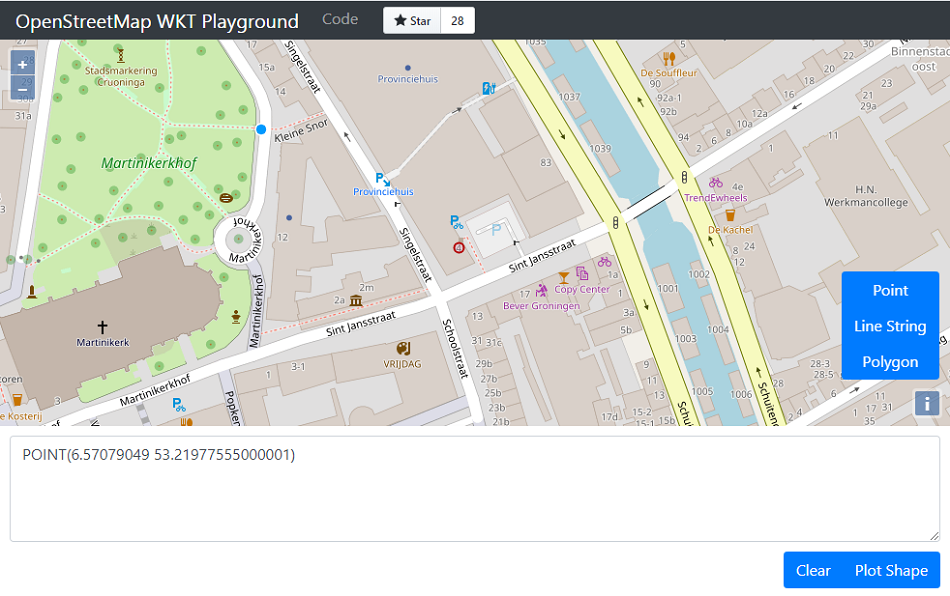
\includegraphics[width=1\linewidth]{images/img01}

Voor adressen is de centroïde gelijk aan de locatie van het adres. Voor andere objecttypen zoals wegen of woonplaatsen is een lijn of vlak misschien beter dan een centroïde. Die wordt opgeslagen in de velden {geometrie\_ll} en {geometrie\_rd}. Ter illustratie vragen we de woonplaatsgrens van Groningen op.

Parameter

Waarde

Beschrijving

{q}

{Groningen}

zoekterm

{rows}

{1}

maximum aantal rijen in de response

{fl}

{weergavenaam,geometrie\_ll,geometrie\_rd}

lijst met velden in de response

{fq}

{type:woonplaats}

filter op de zoekresultaten

Request:\\

De woonplaatsgrens kunnen we bekijken in de \href{https://clydedacruz.github.io/openstreetmap-wkt-playground/}{OpenStreetMap WKT Playground}.

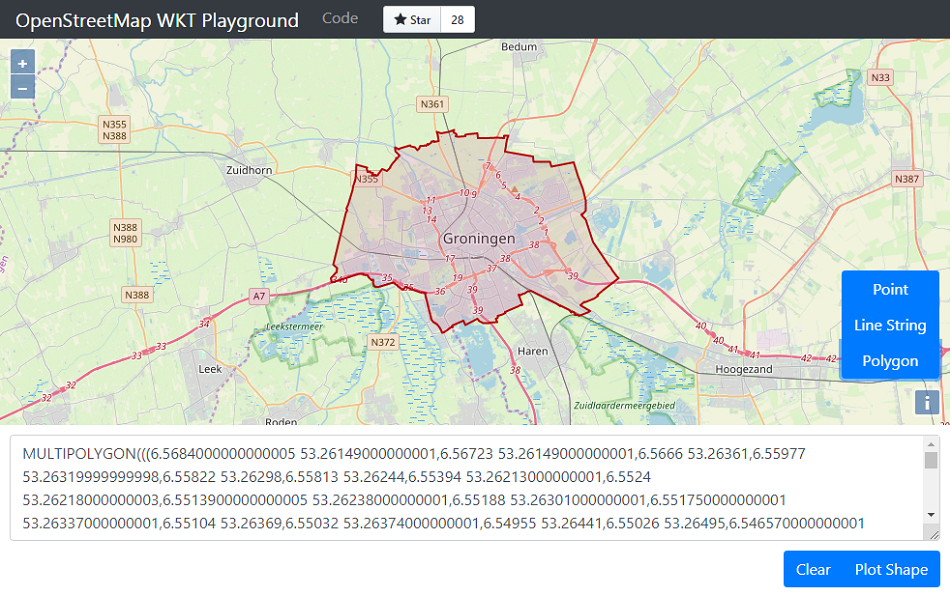
\includegraphics[width=1\linewidth]{images/img02}
Let op: als je een wildcard (*) opgeeft in de {fl} parameter worden {geometrie\_ll} en {geometrie\_rd} niet opgenomen in de response!

Het is overigens ook mogelijk om geometrie in GeoJSON formaat op te vragen. Dit staat beschreven in paragraaf \ref{response-formaat}.

\hypertarget{zoeken-naar-objecten-in-de-buurt}{%
\section{Zoeken naar objecten in de buurt}\label{zoeken-naar-objecten-in-de-buurt}}

\hypertarget{toepassingen}{%
\section{Toepassingen}\label{toepassingen}}

\hypertarget{tips-tricks}{%
\chapter{Tips \& Tricks}\label{tips-tricks}}

In dit hoofdstuk vind je nog wat handige tips voor het werken met LocatieServer.

\hypertarget{postman}{%
\section{Postman}\label{postman}}

\hypertarget{apache-solr}{%
\section{Apache Solr}\label{apache-solr}}

LocatieServer gebruikt \href{https://lucene.apache.org/solr/}{Apache Solr} als search engine. Raadpleeg de \href{https://lucene.apache.org/solr/guide/8_3/searching.html}{Reference Guide} voor meer informatie over zoeken met met Solr.

\hypertarget{debuggen}{%
\section{Debuggen}\label{debuggen}}

Als je tegen problemen aanloopt, kun je de {debug} parameter aan je request toevoegen voor meer informatie.

Met {debug=timing} krijg je bijvoorbeeld informatie over hoe lang het duurde om de query in Solr uit te voeren.

De meest uitgebreide debug informatie krijg je met {debug=all} in je request.

Raadpleeg de Solr documentatie voor meer informatie over de \href{https://lucene.apache.org/solr/guide/8_3/common-query-parameters.html\#debug-parameter}{debug parameter}.

\hypertarget{response-formaat}{%
\section{Response formaat}\label{response-formaat}}

Standaard stuurt LocatieServer de response in {json} formaat terug. Met behulp van de {wt} parameter kun je ook andere formaten specificeren, bijvoorbeeld {xml}.

Een andere optie is {csv}. Je kunt ook parameters toevoegen om het scheidingsteken aan te passen ({csv.separator}) of aan te geven of de response veldnamen moet bevatten ({csv.header}).

Zelfs {geojson} is mogelijk, maar dan moet je ook de parameter {geojson.field} opnemen in het request. De parameter bevat de naam van het veld met de geometrie.

Raadpleeg de Solr documentatie over \href{https://lucene.apache.org/solr/guide/8_3/response-writers.html\#response-writers}{Response Writers} voor meer informatie.

\hypertarget{documentatie}{%
\section{Documentatie}\label{documentatie}}

\begin{itemize}
\tightlist
\item
  \href{https://www.pdok.nl/introductie/-/article/pdok-locatieserver}{LocatieServer API documentatie}
\item
  \href{https://github.com/PDOK/locatieserver/wiki}{LocatieServer wiki}
\end{itemize}

\hypertarget{geoforum}{%
\section{Geoforum}\label{geoforum}}

Het \href{https://geoforum.nl/c/applicaties-en-diensten/locatieserver}{Geoforum} is de beste plek om je vragen over LocatieServer te stellen.

\bibliography{book.bib,packages.bib}


\end{document}
